\section{Dirac-material rates}\label{sec:16.1}

In ZrTe$_5$ the remote bands alone have a dielectric constant of about 50, and the Dirac electrons raise it by \SI{9}{\percent}, to 55 (\cref{we:7-zrte5}). A dark photon that couples to an electron--hole pair in the cone reaches it through both: the field is screened by $|\varepsilon|^2 \approx 3000$, not by the factor $|1 + \varepsilon_{\mathrm{D}}/\varepsilon_{\mathrm{bg}}|^2 = 1.09^2 = 1.2$ that the Dirac electrons contribute alone. The projected reaches of Dirac materials were computed with the second factor~\cite{hochberg2018detection,geilhufe2020dirac}, and for ZrTe$_5$ the two differ by a factor 5200 to 6400 in the scattering rate (\cref{sec:16.1-zrte5}).

\subsection{Loss function of a Dirac target}\label{sec:16.1-loss}

The longitudinal dielectric function is $\varepsilon = 1 - v_{\mathrm{C}}\tilde R$, with $\tilde R$ the proper density response of all the charges (\cref{sec:8.4-proper}). Split $\tilde R = \tilde R_{\mathrm{D}} + \tilde R_{\mathrm{bg}}$ into the Dirac bands inside the cutoff and everything else, the remote bands and, below the optical phonons, the ionic polarization. At energies far below the gap of the remote bands and momenta small compared with the reciprocal lattice, the background responds locally and instantaneously, $1 - v_{\mathrm{C}}\tilde R_{\mathrm{bg}} \to \varepsilon_{\mathrm{bg}}$, real and independent of $\vect{q}$ and $\omega$, with local fields neglected. In the random-phase approximation the proper Dirac response is the independent-pair bubble, $\tilde R_{\mathrm{D}} = R^0_{\mathrm{D}}$, and
\begin{equation}
  \varepsilon(\vect{q},\omega) = \varepsilon_{\mathrm{bg}} + \varepsilon_{\mathrm{D}}(\vect{q},\omega), \qquad \varepsilon_{\mathrm{D}} = -v_{\mathrm{C}}(q)\,R^0_{\mathrm{D}}(\vect{q},\omega) ,
  \label{eq:D.41-eps}
\end{equation}
which is \cref{eq:7.3-epsbg}. By \cref{eq:7.3-eps}, $\varepsilon_{\mathrm{D}} = (g_{\mathrm{deg}}\alpha/6\pi v_{\mathrm{D}})B_{\mathrm{D}}(s)$, with $B_{\mathrm{D}}$ the bracket of that equation: the Coulomb factor $e^2/q^2$ multiplies the bare pair response, and no $\varepsilon_{\mathrm{bg}}$ appears. Since $\varepsilon_{\mathrm{bg}}$ is real, the loss function $L = \Imag(-1/\varepsilon)$ of \cref{eq:4.4-SL} has the Dirac pairs in its numerator and the whole crystal in its denominator. With the spectral form of $R^0_{\mathrm{D}}$ (\cref{eq:2.4-SP}), $\Imag\varepsilon_{\mathrm{D}} = (\pi e^2/q^2)\Vol^{-1}\sum_f|\langle f|n_{\mathrm{D}}(\vect{q})|0\rangle|^2\delta(\omega - \omega_f)$ for $\omega > 0$, the golden-rule sum of pair transitions with a vertex of unit charge.
\begin{keyresult}[Loss function of a Dirac material]
\begin{equation}
  L(\vect{q},\omega) = \frac{\Imag\varepsilon_{\mathrm{D}}}{|\varepsilon_{\mathrm{bg}} + \varepsilon_{\mathrm{D}}|^2} = \frac{g_{\mathrm{deg}}\alpha}{6v_{\mathrm{D}}}\,\frac{\rho(s)\,\Theta(s - 4\Delta_{\mathrm{D}}^2)}{|\varepsilon_{\mathrm{bg}} + \varepsilon_{\mathrm{D}}(\vect{q},\omega)|^2} , \qquad s = \omega^2 - v_{\mathrm{D}}^2q^2 ,
  \label{eq:16.1-L}
\end{equation}
with $\rho(s) = (1 - 4\Delta_{\mathrm{D}}^2/s)^{1/2}(1 + 2\Delta_{\mathrm{D}}^2/s)$ and $\varepsilon_{\mathrm{D}}$ from \cref{eq:7.3-eps}. The scattering rate is \cref{eq:10.2-rate} with this $L$; the absorption rate of a dark photon is \cref{eq:10.7-dp} with $L(0, m_\phi)$.
\end{keyresult}
\noindent For a dark photon, which couples to the total charge, \cref{eq:16.1-L} is exact within the two approximations of \cref{eq:7.3-epsbg}, a local background and the random-phase Dirac response (\cref{eq:8.4-exact}). For a mediator that couples to the electron number it holds with the nuclei clamped. Pairs cost at least $2\Delta_{\mathrm{D}}$, \SI{23.6}{meV} in ZrTe$_5$. Where the pair energies lie above the optical phonons, $\varepsilon_{\mathrm{bg}}$ is the clamped-ion constant of the remote bands. Near a polar phonon it acquires the ionic poles of \cref{sec:5.5} and depends on $\omega$.

The numerator of \cref{eq:16.1-L} does not depend on the background. Deep in the continuum it is $g_{\mathrm{deg}}\alpha/6v_{\mathrm{D}}$, which is 6.1 for $v_{\mathrm{D}} = 4\times10^{-4}$, and all of the dependence on $\varepsilon_{\mathrm{bg}}$ sits in the denominator. At weak screening, $|\varepsilon_{\mathrm{D}}| \ll \varepsilon_{\mathrm{bg}}$, the loss function tends to the leading form $\Imag\varepsilon_{\mathrm{D}}/\varepsilon_{\mathrm{bg}}^2$, and the rate of a Dirac target falls as $1/(v_{\mathrm{D}}\varepsilon_{\mathrm{bg}}^2)$. The factor $|1 + \varepsilon_{\mathrm{D}}/\varepsilon_{\mathrm{bg}}|^{-2}$ that separates the two forms is the screening by the Dirac electrons themselves, the charge renormalization of quantum electrodynamics with $v_{\mathrm{D}}$ in place of the speed of light. Its size is set by $g_{\mathrm{deg}}\tilde\alpha$, with $\tilde\alpha = \alpha/(\varepsilon_{\mathrm{bg}}v_{\mathrm{D}})$ the effective coupling of \cref{eq:7.3-alpha}, times a logarithm: 0.61 at a pair energy of \SI{10}{meV} in the benchmark of \cref{we:16-factor}, and 0.86 to 0.94 for the rate of ZrTe$_5$.

The inputs are those of \cref{sec:7.3}: the principal velocities, the half-gap, the cutoff and the background tensor. Their values for ZrTe$_5$, and the excitonic calculation that the threshold region needs, are specified in \cref{app:E.20}. A computed dielectric tensor contains the Dirac pairs, which the background must exclude (\cref{sec:7.3}); for ZrTe$_5$ the Dirac part is 3 to \SI{8}{\percent} of each component for the parameters used below (\cref{we:16-band}), within the spread of the computed tensors.

\subsection{Background screening in the published rates}\label{sec:16.1-published}\label{app:D.41}

The published Dirac rates~\cite{hochberg2018detection,geilhufe2020dirac} are assembled differently. The reference cross-section $\sigmae$ is defined in vacuum, from the free amplitude~\cite[Eqs.~(3.8), (3.10), (3.11)]{hochberg2018detection}, \cite[Eqs.~(2.3), (2.4)]{geilhufe2020dirac}. The pair transitions are summed with the same unit-charge vertex, through the overlap of the band spinors. The medium enters through the in-medium form factor $F_{\mathrm{med}} = 1/\varepsilon_{\mathrm{pub}}$, where $\varepsilon_{\mathrm{pub}} = 1 + \varepsilon_{\mathrm{D}}/\varepsilon_{\mathrm{bg}}$ (written $\varepsilon_r$ there) is the polarization of the Dirac electrons alone, computed with the charge $e/\varepsilon_{\mathrm{bg}}^{1/2}$ in the loop and the vacuum photon propagator outside it~\cite[Eqs.~(2.5), (2.6), (3.7), (3.11), (A.8)]{hochberg2018detection}, \cite[Eqs.~(2.5)--(2.7), (3.3)]{geilhufe2020dirac}. Since $\varepsilon_{\mathrm{pub}} = \varepsilon/\varepsilon_{\mathrm{bg}}$, the background screens the Dirac electrons among themselves but not the field of the dark photon. For absorption the same polarization serves as the photon self-energy, $\Pi = \omega^2(1 - \varepsilon_{\mathrm{pub}})$~\cite[Eqs.~(4.4), (4.5)]{hochberg2018detection}, \cite[Eqs.~(2.25)--(2.27)]{geilhufe2020dirac}. Then $\zeta_{\mathrm{eff}}^2 = \zeta^2/|\varepsilon_{\mathrm{pub}}|^2$ by \cref{eq:8.4-zetaeff}, and $-\Imag\Pi/\omega = m_\phi\Imag\varepsilon_{\mathrm{pub}} = m_\phi\Imag\varepsilon_{\mathrm{D}}/\varepsilon_{\mathrm{bg}}$.
\begin{keyresult}[Published Dirac rates against the total $\varepsilon$]
For an isotropic Dirac material, at every $(\vect{q},\omega)$ and for any size of $\varepsilon_{\mathrm{D}}$,
\begin{equation}
  L_{\mathrm{pub}} = \frac{\Imag\varepsilon_{\mathrm{D}}}{|\varepsilon/\varepsilon_{\mathrm{bg}}|^2} = \varepsilon_{\mathrm{bg}}^2\,L , \qquad
  \varGamma_{\mathrm{pub}} = \zeta^2m_\phi\,\frac{\Imag\varepsilon_{\mathrm{pub}}}{|\varepsilon_{\mathrm{pub}}|^2} = \varepsilon_{\mathrm{bg}}\,\varGamma ,
  \label{eq:16.1-ratio}
\end{equation}
so that a background-free reach curve moves by $\sigmae^{\mathrm{lim}} \to \varepsilon_{\mathrm{bg}}^2\sigmae^{\mathrm{lim}}$ and $\zeta^{\mathrm{lim}} \to \varepsilon_{\mathrm{bg}}^{1/2}\zeta^{\mathrm{lim}}$ at every mass. For an anisotropic material the factors hold along the principal axes, with $\varepsilon_{\mathrm{bg},ii}$.
\end{keyresult}
\noindent The powers differ because the numerators differ. In scattering the numerator is the bare pair spectrum with the vacuum charge, while in absorption $\Imag\varepsilon_{\mathrm{pub}} = \Imag\varepsilon_{\mathrm{D}}/\varepsilon_{\mathrm{bg}}$ already carries one $1/\varepsilon_{\mathrm{bg}}$, the square of the reduced charge in the loop. The published curves keep the real part of $\varepsilon_{\mathrm{D}}$ in $|\varepsilon_{\mathrm{pub}}|^2$, so the shifts of the reach need no further factor. A recomputation that keeps only the leading term of \cref{eq:16.1-L} at weak screening, $L \to \Imag\varepsilon_{\mathrm{D}}/\varepsilon_{\mathrm{bg}}^2$, must restore the factor $|1 + \varepsilon_{\mathrm{D}}/\varepsilon_{\mathrm{bg}}|^{-2}$ instead, and applying both would count the screening by the Dirac electrons twice.

The published loss function has an exact physical meaning. Let a field couple to the Dirac electrons and to no other charge. Its potential induces a Dirac charge, whose Coulomb field, screened by the background, acts back on the Dirac electrons with $v_{\mathrm{C}}/\varepsilon_{\mathrm{bg}}$; the random-phase sum of this chain is $R_{\mathrm{DD}} = R^0_{\mathrm{D}}/(1 - v_{\mathrm{C}}R^0_{\mathrm{D}}/\varepsilon_{\mathrm{bg}}) = R^0_{\mathrm{D}}/\varepsilon_{\mathrm{pub}}$. Because $R^0_{\mathrm{D}}\varepsilon_{\mathrm{pub}}^* = R^0_{\mathrm{D}} - v_{\mathrm{C}}|R^0_{\mathrm{D}}|^2/\varepsilon_{\mathrm{bg}}$ has the imaginary part $\Imag R^0_{\mathrm{D}}$, $-v_{\mathrm{C}}\Imag R_{\mathrm{DD}} = \Imag\varepsilon_{\mathrm{D}}/|\varepsilon_{\mathrm{pub}}|^2 = L_{\mathrm{pub}}$. The published rate is therefore the rate of a mediator that couples to the Dirac electrons alone, whereas a kinetically mixed dark photon couples to the electromagnetic current, remote bands included~\cite[Eq.~(2.1)]{hochberg2018detection}.

The factor $\varepsilon_{\mathrm{bg}}^2$ is not an artifact of the cutoff. For a gapless cone with a hard cutoff, \cref{eq:D.22-gapless} gives $\varepsilon/\varepsilon_{\mathrm{bg}} = 1 + (g_{\mathrm{deg}}\tilde\alpha/6\pi)[\ln(4v_{\mathrm{D}}^2\Lambda_{\mathrm{D}}^2/|s|) + \ii\pi\Theta(s)]$ with $s = \omega^2 - v_{\mathrm{D}}^2q^2$. The constant 1 can be absorbed into the cutoff, $\Lambda' = \Lambda_{\mathrm{D}}\exp[3\pi/(g_{\mathrm{deg}}\tilde\alpha)]$, and then $\varepsilon/\varepsilon_{\mathrm{bg}} = (g_{\mathrm{deg}}\tilde\alpha/6\pi)\mathcal{L}'$ with $\mathcal{L}' = \ln(4v_{\mathrm{D}}^2\Lambda'^2/|s|) + \ii\pi\Theta(s)$, an identity. It holds in either subtraction scheme, since the constant $\tfrac53$ by which the schemes differ is absorbed into $\Lambda'$ in the same way. It gives
\begin{equation}
  \frac{1}{|\varepsilon|^2} = \Bigl(\frac{6\pi v_{\mathrm{D}}}{g_{\mathrm{deg}}\alpha}\Bigr)^2\frac{1}{|\mathcal{L}'|^2} , \qquad
  \frac{1}{|\varepsilon_{\mathrm{pub}}|^2} = \Bigl(\frac{6\pi\varepsilon_{\mathrm{bg}}v_{\mathrm{D}}}{g_{\mathrm{deg}}\alpha}\Bigr)^2\frac{1}{|\mathcal{L}'|^2} .
  \label{eq:D.41-lprime}
\end{equation}
In the total-$\varepsilon$ rate the prefactor $g_{\mathrm{deg}}\tilde\alpha\varepsilon_{\mathrm{bg}} = g_{\mathrm{deg}}\alpha/v_{\mathrm{D}}$ does not depend on the background; in the published rate it carries $\varepsilon_{\mathrm{bg}}^2$ explicitly. The rescaled cutoff is that of Ref.~\cite[text after Eq.~(3.13)]{hochberg2018detection}, $\Lambda' = \Lambda\exp[12\pi^2\varepsilon_{\mathrm{bg}}v_{\mathrm{D}}/(g_{\mathrm{deg}}e^2)]$, and the prefactor $288\pi^4\varepsilon_{\mathrm{bg}}^2v_{\mathrm{D}}^2/(e^4g_{\mathrm{deg}}^2)$ of its Eq.~(3.13) is $\frac12(6\pi\varepsilon_{\mathrm{bg}}v_{\mathrm{D}}/g_{\mathrm{deg}}\alpha)^2$: the explicit $\varepsilon_{\mathrm{bg}}^2$ in it is the omitted $1/\varepsilon_{\mathrm{bg}}^2$. At large $\varepsilon_{\mathrm{bg}}$, $|\mathcal{L}'| \approx 6\pi/(g_{\mathrm{deg}}\tilde\alpha) \propto \varepsilon_{\mathrm{bg}}$, so the published rate tends to a constant, the unscreened rate of the Dirac pairs, while the total-$\varepsilon$ rate falls as $1/\varepsilon_{\mathrm{bg}}^2$.

How large is the factor in a material where the one-loop dielectric function can be trusted? For an isotropic cone, or along a principal axis with $v_i$ and $\varepsilon_{\mathrm{bg},ii}$ in place of $v_{\mathrm{D}}$ and $\varepsilon_{\mathrm{bg}}$, scattering needs $v_{\mathrm{D}} < v_{\mathrm{max}}$ (\cref{sec:7.3}), and the weak-coupling condition $\tilde\alpha = \alpha/(\varepsilon_{\mathrm{bg}}v_{\mathrm{D}}) < 1$ then requires $\varepsilon_{\mathrm{bg}} > \alpha/v_{\mathrm{D}} > \alpha/v_{\mathrm{max}} = 2.75$. Wherever both hold, the published scattering rate is too large by at least $(\alpha/v_{\mathrm{max}})^2 = 7.6$, and for a cone slower than $v_{\mathrm{max}}$ the published absorption rate, too large by $\varepsilon_{\mathrm{bg}}$, by at least $\alpha/v_{\mathrm{max}} = 2.75$; absorption needs no $v_{\mathrm{D}} < v_{\mathrm{max}}$, and a faster cone has a smaller bound $\alpha/v_{\mathrm{D}}$. The published form is the $\varepsilon_{\mathrm{bg}} \to 1$ limit of \cref{eq:16.1-L}, and \cref{lim:16.1a} follows the two rates as the background grows.

The correction also reverses a rule for choosing a target. In the published form the scattering rate grows with $\varepsilon_{\mathrm{bg}}$ toward the unscreened rate of the pairs, and the absorption rate $\propto \varepsilon_{\mathrm{bg}}\Imag\varepsilon_{\mathrm{D}}/|\varepsilon_{\mathrm{bg}} + \varepsilon_{\mathrm{D}}|^2$ is largest at $\varepsilon_{\mathrm{bg}} = |\varepsilon_{\mathrm{D}}|$, with $|\varepsilon_{\mathrm{D}}| = 7.6$ at \SI{50}{meV} in the material of \cref{lim:16.1a}. A maximum of this kind underlies the optimal ratio $\varepsilon_{\mathrm{bg}}/g_{\mathrm{deg}} \sim 10$ found by Hochberg et al.~\cite[Sect.~4.2]{hochberg2018detection}. With the total $\varepsilon$ both rates fall monotonically as the background grows at fixed Dirac parameters. The best Dirac target has the smallest background constant that still keeps the coupling weak, $\varepsilon_{\mathrm{bg}}$ near $\alpha/v_{\mathrm{D}}$.

\begin{limitbox}[Background screening of Dirac-material rates][lim:16.1a]
Published scattering and absorption rates of a Dirac material, with the vacuum $\sigmae$ and the in-medium factor $1/\varepsilon_{\mathrm{pub}}$~\cite[Eqs.~(3.7), (3.11), (4.4), (4.5)]{hochberg2018detection}, \cite[Eqs.~(2.7), (2.25)--(2.27), (3.14)]{geilhufe2020dirac}: the $\varepsilon_{\mathrm{bg}} \to 1$ limit of \cref{eq:16.1-L} and \cref{eq:10.7-dp}.
\par\smallskip
{\centering
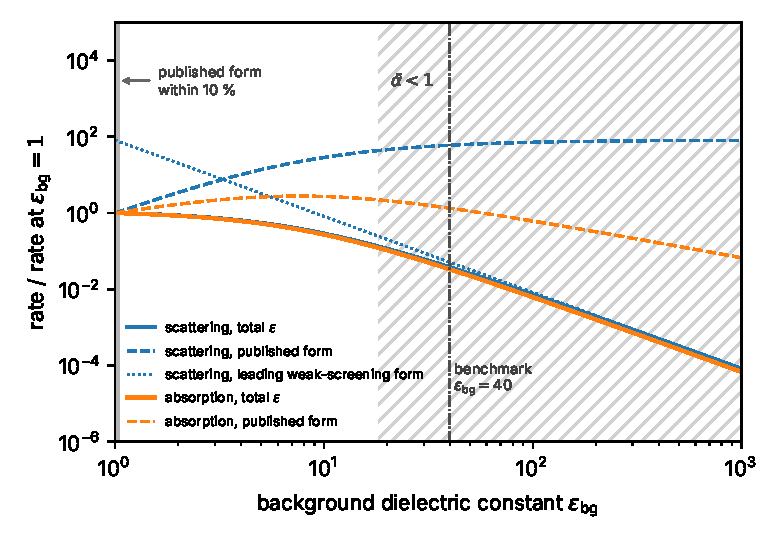
\includegraphics[width=0.9\linewidth]{figures/ch16/limit16_1a.pdf}
\captionof{figure}{Rates of the gapped isotropic Dirac material of Ref.~\cite{hochberg2018detection} ($v_{\mathrm{D}} = 4\times10^{-4}$, $\Delta_{\mathrm{D}} = \SI{2.5}{meV}$, $g_{\mathrm{deg}} = 2$, hard cutoff $\Lambda_{\mathrm{D}} = \SI{0.2}{keV}$) against the background dielectric constant at fixed Dirac parameters, each divided by its value at $\varepsilon_{\mathrm{bg}} = 1$, where the two forms coincide. Blue: scattering at $m_\chi = \SI{100}{keV}$ through a light mediator, \cref{eq:10.2-rate}, with the total $\varepsilon$ (solid), the published form (dashed) and the leading weak-screening form $\Imag\varepsilon_{\mathrm{D}}/\varepsilon_{\mathrm{bg}}^2$ (dotted). Orange: dark-photon absorption at $m_\phi = \SI{50}{meV}$ with the total $\varepsilon$ (solid) and the published form (dashed). Gray: $\varepsilon_{\mathrm{bg}} \le 1.049$, where the published scattering rate is within \SI{10}{\percent} of the total-$\varepsilon$ rate. Hatched: $\tilde\alpha < 1$, $\varepsilon_{\mathrm{bg}} > \alpha/v_{\mathrm{D}} = 18.2$, where one-loop screening is used. Dash-dotted: the published benchmark $\varepsilon_{\mathrm{bg}} = 40$, where the total-$\varepsilon$ scattering rate is 0.74 of its leading form. The dashed curves are $\varepsilon_{\mathrm{bg}}^2$ and $\varepsilon_{\mathrm{bg}}$ times the solid ones.}\label{fig:16-limit-dirac}
\par}
\smallskip
For $\varepsilon_{\mathrm{bg}} > 1$ the published form leaves out the screening of the dark-photon field by the remote bands; at large $\varepsilon_{\mathrm{bg}}$ its scattering rate tends to the unscreened rate of the Dirac pairs, 0.99 of it at $\varepsilon_{\mathrm{bg}} = 1000$, while the true rate falls as $1/\varepsilon_{\mathrm{bg}}^2$.
\end{limitbox}

\begin{workedexample}{The factor $\varepsilon_{\mathrm{bg}}^2$ at $\varepsilon_{\mathrm{bg}} = 40$}\label{we:16-factor}
The ideal Dirac material of Ref.~\cite[Fig.~4]{hochberg2018detection} has $v_{\mathrm{D}} = 4\times10^{-4}$, $\varepsilon_{\mathrm{bg}} = 40$, $g_{\mathrm{deg}} = 2$ and a cutoff of \SI{0.2}{keV}, which we read as a hard cutoff, $v_{\mathrm{D}}\Lambda_{\mathrm{D}} = \SI{80}{meV}$. The coupling is $\tilde\alpha = \alpha/(40\times4\times10^{-4}) = 0.456$, and $g_{\mathrm{deg}}\tilde\alpha = 0.91$ is the effective coupling quoted there.

\emph{One point.} Take the gapless cone at $\vect{q} \to 0$ and $\omega = \SI{10}{meV}$, so that $\sqrt{s} = \SI{10}{meV}$. \Cref{eq:D.22-gapless} gives the bracket $\ln(4v_{\mathrm{D}}^2\Lambda_{\mathrm{D}}^2/s) + \ii\pi = 5.545 + 3.142\ii$, and with $g_{\mathrm{deg}}\alpha/(6\pi v_{\mathrm{D}}) = 1.936$, $\varepsilon_{\mathrm{D}} = 10.73 + 6.08\ii$. The total is $\varepsilon = 50.73 + 6.08\ii$ and $|\varepsilon|^2 = 2611$, so $L = 6.08/2611 = 2.33\times10^{-3}$, 0.61 of the leading form $6.08/1600 = 3.80\times10^{-3}$. Had the \SI{0.2}{keV} been a cutoff in the subtraction scheme of the reference, the bracket would gain $\frac53$, $\Real\varepsilon_{\mathrm{D}}/\varepsilon_{\mathrm{bg}}$ would rise from 0.27 to 0.35, and the ratio to the leading form would be 0.54. The published construction divides $\Imag\varepsilon_{\mathrm{D}} = 6.08$ by $|\varepsilon/\varepsilon_{\mathrm{bg}}|^2 = 1.632$ and obtains 3.73, which is $1600$ times $L$.

\emph{Absorption.} At $m_\phi = \SI{10}{meV}$ the same $\varepsilon$ applies. The published rate is $\zeta^2m_\phi\Imag\varepsilon_{\mathrm{pub}}/|\varepsilon_{\mathrm{pub}}|^2 = 0.0932\,\zeta^2m_\phi$, forty times $\zeta^2m_\phi L$. With the density \SI{10}{g.cm^{-3}} of the reference and $\rho_\chi = \SI{0.3}{GeV.cm^{-3}}$, \cref{eq:10.7-dp} gives $3.35\times10^{30}\,\zeta^2$ events per kg-year, and three events in a kg-year reach $\zeta = 9.5\times10^{-16}$, against $1.5\times10^{-16}$ with the published form, a factor $\sqrt{40} = 6.3$.

\emph{Scattering reach.} For scattering the reference counts one Dirac valence electron per cell, $n_e = \SI{5e24}{kg^{-1}}$ electrons per unit mass in cells of $V_{\mathrm{uc}} = \SI{60}{\angstrom^3}$, which fixes the density $1/(n_eV_{\mathrm{uc}}) = \SI{3.33}{g.cm^{-3}}$; its absorption estimate takes \SI{10}{g.cm^{-3}} instead, and we keep each with its own rate. For the gapped cone ($\Delta_{\mathrm{D}} = \SI{2.5}{meV}$) at $m_\chi = \SI{100}{keV}$, with the standard halo and three events in a kg-year, \cref{eq:10.2-rate} with \cref{eq:16.1-L} reaches $\sigmae = \SI{4.4e-42}{cm^2}$, and the published form $\SI{2.8e-45}{cm^2}$, a factor 1600 at this and at every other mass, 3.2 decades. The published curve for this material has its minimum, \SI{3.4e-46}{cm^2} near \SI{9}{keV}, read from the reference's figure; corrected, it lies at \SI{5.4e-43}{cm^2}.\footnote{The published curve lies about a factor two above the reference's own formula: with the standard halo it reads \SI{5.0e-45}{cm^2} at \SI{100}{keV} against the recomputed \SI{2.8e-45}{cm^2}, a factor 1.8. The factor 1600 between the published and the total-$\varepsilon$ reach holds either way.}
\end{workedexample}

\subsection{ZrTe\texorpdfstring{$_5$}{5} and other anisotropic targets}\label{sec:16.1-zrte5}

Take an anisotropic cone and a background tensor with the same principal axes. The background enters the longitudinal function as $\hat{\vect{q}}\cdot\varepsilon_{\mathrm{bg}}\cdot\hat{\vect{q}} = \sum_i\varepsilon_{\mathrm{bg},ii}\hat q_i^2$. The rescaling at the end of \cref{app:D.22} turns $q^2/v_{\mathrm{D}}$ in the overlap into $\tilde q^2/(v_1v_2v_3)$ with $\tilde{\vect{q}} = (v_1q_1, v_2q_2, v_3q_3)$, so that
\begin{equation}
  \varepsilon(\vect{q},\omega) = \sum_i\varepsilon_{\mathrm{bg},ii}\hat q_i^2 + \sum_i\hat q_i^2\,\varepsilon_{\mathrm{D},i}(\omega^2 - \tilde q^2), \qquad
  \varepsilon_{\mathrm{D},i} = \frac{g_{\mathrm{deg}}\alpha}{6\pi}\,\frac{v_i^2}{v_1v_2v_3}\,B_{\mathrm{D}}(\omega^2 - \tilde q^2) ,
  \label{eq:D.41-aniso}
\end{equation}
with $B_{\mathrm{D}}$ the bracket of \cref{eq:7.3-eps} and $v_{\mathrm{D}}\Lambda_{\mathrm{D}}$ replaced by the energy cutoff $\tilde\Lambda$ of \cref{eq:7.3-aniso}. Both terms of \cref{eq:D.41-aniso} carry the factor $\hat q_i^2$ of a longitudinal function; the background is not divided into the Dirac term. The in-medium factor of Ref.~\cite[Eq.~(3.14)]{geilhufe2020dirac} instead divides each component of the Dirac polarization by its own background constant, $\varepsilon_{\mathrm{pub}} = 1 + \sum_i\hat q_i^2\varepsilon_{\mathrm{D},i}/\varepsilon_{\mathrm{bg},ii}$. The ratio of the two loss functions is
\begin{equation}
  \frac{L_{\mathrm{pub}}}{L} = \frac{|\sum_i\hat q_i^2(\varepsilon_{\mathrm{bg},ii} + \varepsilon_{\mathrm{D},i})|^2}{|1 + \sum_i\hat q_i^2\varepsilon_{\mathrm{D},i}/\varepsilon_{\mathrm{bg},ii}|^2} .
  \label{eq:D.41-ratio}
\end{equation}
(The term of the $x$ axis is read with $q_x^2v_x^2$, where that equation prints $q_x^2v_z^2$.) Along a principal axis the ratio is $\varepsilon_{\mathrm{bg},ii}^2$, which for the computed tensor of ZrTe$_5$, $\varepsilon_{\mathrm{bg},ii} = 308.4$, 20.75 and 126.1~\cite[Table~2]{geilhufe2020dirac}, is $9.5\times10^4$, 431 and $1.6\times10^4$. Off the axes it is not a power of any single background constant: for $\varepsilon_{\mathrm{D}} \to 0$ it tends to $(\hat{\vect{q}}\cdot\varepsilon_{\mathrm{bg}}\cdot\hat{\vect{q}})^2$, and for finite $\varepsilon_{\mathrm{D}}$ it depends on $\hat{\vect{q}}$ through both sums. The event rates then differ by the ratio of their integrals over directions and energies, which the reach of an anisotropic target must be computed with. The background tensor also orders the directions by itself. At equal Dirac numerator, a momentum transfer along $y$, the axis of the smallest background constant, gives a rate $(308.4/20.75)^2 = 221$ times that along $x$. The rate of a crystal fixed in the laboratory therefore modulates daily mainly through its background tensor, which neither a harmonic mean of the tensor nor the per-component factor represents.

We evaluate ZrTe$_5$ with the parameter row that the calculation of \cref{we:7-zrte5} gives for the measured crystal structure~\cite[Table~1 and text below it]{geilhufe2020dirac}: the principal velocities $1.1\times10^{-3}$, $4.5\times10^{-4}$ and $1.0\times10^{-3}$, the energy cutoff $\tilde\Lambda = \min_iv_i\Lambda_i = \SI{0.191}{eV}$, $g_{\mathrm{deg}} = 2$, and the half-gap $\Delta_{\mathrm{D}} = \SI{11.8}{meV}$, half the computed gap of \SI{23.6}{meV}. The relaxed cell of \cref{we:7-zrte5}, the row the reference implements, gives \SI{15.6}{meV} with its own velocities and cutoff, and an earlier calculation \SI{17.5}{meV}. The threshold mass is \SI{8.0}{keV} for the isotropic cone and 9.6, 7.1 and \SI{9.0}{keV} along the principal axes. We average the loss function over the directions of $\vect{q}$, which gives the rate averaged over the orientations of the crystal relative to the dark-matter wind, and insert it into \cref{eq:10.2-rate} with a light mediator, the standard halo and the measured density \SI{6.089}{g.cm^{-3}}~\cite[Fig.~3]{geilhufe2020dirac}. At $m_\chi = \SI{100}{keV}$ and $\sigmae = \SI{e-38}{cm^2}$ this yields 108 events per kg-year. Since a background-free reach scales as the inverse rate (\cref{eq:1.5-limscaling}), three events in a kg-year reach about \SI{1.5e-40}{cm^2} near \SI{40}{keV} (\cref{fig:16-zrte5}a). The published rule, recomputed with the same inputs and the standard halo, gives a rate 5200 to 6400 times larger between \SI{20}{keV} and \SI{1}{MeV}. Over the two computed rows (11.8 and \SI{15.6}{meV}) and the two halos of \cref{fig:16-zrte5} the factor spans 4800 to 6600, and a halo with $v_0 = 220$, $v_{\mathrm{E}} = 232$ and $v_{\mathrm{esc}} = \SI{544}{km.s^{-1}}$ lowers its lower end to 4300. That is more than the square of the harmonic mean of the tensor, $50.5^2 = 2550$, and an isotropic model of the same row, with the geometric-mean velocity and the harmonic-mean background as in \cref{we:7-zrte5}, overstates the orientation-averaged total-$\varepsilon$ rate by a factor 2.3 to 2.7. The curve of Hochberg et al.~\cite{hochberg2018detection}, computed for an isotropic model with $\varepsilon_{\mathrm{bg}} = 25.34$, the harmonic mean of its own tensor (187.5, 9.8 and 90.9), moves by $25.34^2 = 642$ exactly.

\begin{figure}[tbp]
  \centering
  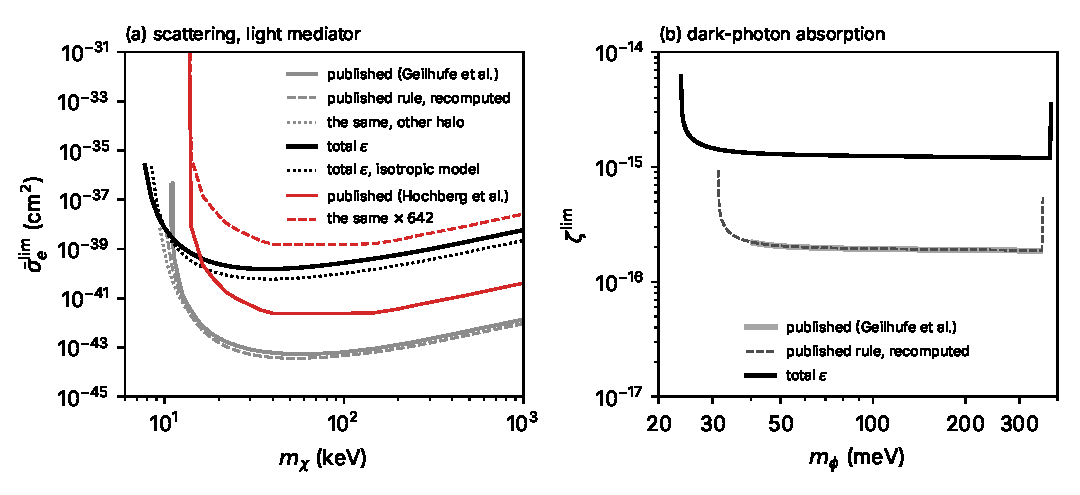
\includegraphics[width=\linewidth]{figures/ch16/fig16_1.pdf}
  \caption{ZrTe$_5$ reach as published and with the background in the total dielectric function: three events in one kg-year, no background, $\rho_\chi = \SI{0.3}{GeV.cm^{-3}}$. (a) Scattering through a light mediator. Gray solid: the published curve for the computed parameters of Geilhufe et al.~\cite{geilhufe2020dirac} (read from their figure). Gray dashed: their in-medium factor, recomputed for their half-gap, \SI{15.6}{meV}, with the standard halo and the loss function averaged over the directions of $\vect{q}$; it lies at 0.63 to 0.72 of the published curve above \SI{20}{keV}, consistent with a difference of halo: the source states none, and with $v_0 = 220$, $v_{\mathrm{E}} = 232$ and $v_{\mathrm{esc}} = \SI{600}{km.s^{-1}}$ (gray dotted) the ratio is 0.8 to 1.1. Black solid: the target with the total $\varepsilon$, \cref{eq:16.1-L} with the anisotropic $\varepsilon_{\mathrm{D}}$ of \cref{eq:D.41-aniso}, measured-structure row ($\Delta_{\mathrm{D}} = \SI{11.8}{meV}$, $\tilde\Lambda = \SI{0.191}{eV}$), density \SI{6.089}{g.cm^{-3}}. Black dotted: its isotropic model (geometric-mean velocity, harmonic-mean $\varepsilon_{\mathrm{bg}} = 50.5$) with the total $\varepsilon$. Red: the published curve of Hochberg et al.~\cite{hochberg2018detection} for their ZrTe$_5$ parameters, isotropized with $\varepsilon_{\mathrm{bg}} = 25.34$ (solid), and the same curve times 642 (dashed). (b) Absorption of dark-photon dark matter, each polarization along a principal axis, unpolarized average, density \SI{6.135}{g.cm^{-3}} as in Ref.~\cite{geilhufe2020dirac}. Gray: their published curve; dashed: their rule recomputed with $\Delta_{\mathrm{D}} = \SI{15.6}{meV}$, within \SI{0.5}{\percent} of it; black: the total $\varepsilon$ with the measured-structure row. Published-rule curves: $\Delta_{\mathrm{D}} = \SI{15.6}{meV}$, $\tilde\Lambda = \SI{0.180}{eV}$. Off-diagonal entries of the tensor ($|\varepsilon_{\mathrm{bg},ij}| \le 1.2$) are dropped.}
  \label{fig:16-zrte5}
\end{figure}

Absorption at rest has no direction of $\vect{q}$, but the polarization of the dark photon picks a component of the tensor, and each polarization is absorbed with the factor $\varepsilon_{\mathrm{bg},ii}$ of \cref{eq:16.1-ratio}. With the total $\varepsilon$ the polarization along $y$, with the smallest background constant, carries \SI{86}{\percent} of the unpolarized rate at \SI{100}{meV}. Recomputed with the published rule, our absorption rate reproduces the published reach of Ref.~\cite{geilhufe2020dirac} to \SI{0.5}{\percent} over the whole range, which checks the inputs. With the total $\varepsilon$ and the measured-structure row, the reach in $\zeta$ weakens by a factor of 6.3 to 6.4 between the gap and the cutoff (\cref{fig:16-zrte5}b), to about $1.25\times10^{-15}$ at \SI{100}{meV}. The factor is the square root of a polarization average and lies between $\varepsilon_{\mathrm{bg},yy}^{1/2} = 4.6$ and $\varepsilon_{\mathrm{bg},xx}^{1/2} = 17.6$. For the cubic Yb$_3$PbO of the same reference the factors are $42.8^2 = 1832$ and $42.8^{1/2} = 6.5$ identically. Its computed dielectric constant, however, is described there as sensitive to the size of the gap~\cite[Sect.~4]{geilhufe2020dirac}. It contains the Dirac bands, the background is smaller than 42.8, and the Dirac term is counted twice under either rule. These two factors describe the model, not the material.

\subsection{Excitonic and strong-coupling corrections}\label{sec:16.1-validity}

\Cref{eq:16.1-L} keeps the random-phase response of the Dirac electrons, the first order in $\tilde\alpha$ of their polarization, with the expansion parameter $g_{\mathrm{deg}}\tilde\alpha\ln[v_{\mathrm{D}}\Lambda_{\mathrm{D}}/\max(\Delta_{\mathrm{D}}, v_{\mathrm{D}}q)]$ of \cref{sec:7.3}. For ZrTe$_5$ that is 1.02 at long wavelength with the measured-structure row (0.93 with the relaxed cell), at the edge of the expansion, and for the benchmark of \cref{we:16-factor}, $g_{\mathrm{deg}}\tilde\alpha = 0.91$ times a logarithm of a few. At next order the electron--hole ladder, the self-energy and vertex of the carriers, and the material outside the model all enter.

The ladder of the Bethe--Salpeter equation (\cref{sec:4.9}) is the attraction between the electron and the hole of a pair. Near the edge the pair is nonrelativistic, with reduced mass $\Delta_{\mathrm{D}}/2v_{\mathrm{D}}^2$ and Coulomb coupling $\alpha/\varepsilon_{\mathrm{bg}}$. It binds with the energy $(\Delta_{\mathrm{D}}/2v_{\mathrm{D}}^2)(\alpha/\varepsilon_{\mathrm{bg}})^2/2 = \Delta_{\mathrm{D}}\tilde\alpha^2/4$, \SI{0.10}{meV} for the isotropic model of ZrTe$_5$ with $\tilde\alpha = 0.18$, and its continuum carries the Sommerfeld factor $x/(1 - \ee^{-x})$ with $x = \pi\tilde\alpha/b$. Here $b = (1 - 4\Delta_{\mathrm{D}}^2/s)^{1/2}$ is the speed of each carrier in the rest frame of the pair, in units of $v_{\mathrm{D}}$. In ZrTe$_5$ the factor exceeds 1.5 for $b < 0.66$, that is for pair energies up to 1.33 times the edge, and that region carries \SI{60}{\percent} of the rate at \SI{20}{keV}, \SI{12}{\percent} at \SI{100}{keV} and \SI{3}{\percent} at \SI{1}{MeV} in the isotropic model. Near the threshold mass the reach is therefore uncertain by the Sommerfeld factor, 1.5 or more, until the ladder is solved, which \cref{app:E.20} specifies. The bound states lie at $\sqrt{s} < 2\Delta_{\mathrm{D}}$ and add absorption lines below the edge.

The self-energy of the carriers renormalizes $v_{\mathrm{D}}$ logarithmically in the cutoff, and a vertex correction accompanies it. Each is of relative order $\tilde\alpha$, with a coefficient that the one-loop result does not fix. Outside the model, a chemical potential inside a band adds an intraband term, Thomas--Fermi screening with $k_{\mathrm{TF}}^2 = e^2\mathcal{N}_{\mathrm{D}}(E_{\mathrm{F}})/\varepsilon_{\mathrm{bg}}$, which removes the weak screening at $\omega \lesssim v_{\mathrm{D}}k_{\mathrm{F}}$. The background acquires ionic poles near the optical phonons. And the bands bend beyond $\Lambda_{\mathrm{D}}$, which moves weight between the background and the logarithm of \cref{eq:7.3-static}.

At $\tilde\alpha \gtrsim 1$ none of these is small, and no controlled method is known. The ladder is the controlled correction of first order in $\tilde\alpha$ and is uncontrolled beyond it; neither self-consistent $GW$ with the Bethe--Salpeter equation nor a functional renormalization group has a small parameter there. The question matters for the slowest cones, which have the most states and the lowest thresholds. BNQ-TTF, with velocities near $2\times10^{-4}$, has an effective coupling of about 10, and its authors present its one-loop rates as a qualitative estimate~\cite[footnote~3]{geilhufe2020dirac}. What replaces \cref{eq:16.1-L} for such targets is open.
